%\part{Konstruktion}
%\chapter{Programmlogik}
%\section{QueryResolution}

\subsection{QuerySend}

\begin{figure}[htb]
  	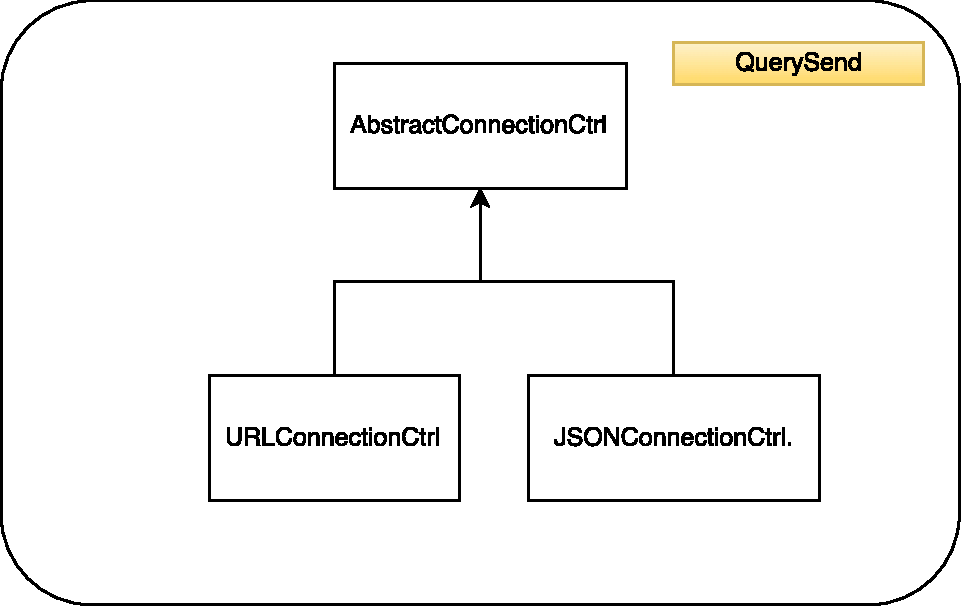
\includegraphics[width=\textwidth]{qr_querysend}
  	\caption{Aufbau des Moduls \lstinline|QuerySend|}
	\label{fig:Aufbau des Moduls \lstinline|QuerySend|}
\end{figure}

Im Modul \lstinline|QuerySend| befinden sich die \lstinline|ConnectionController|, welche für das Versenden der Anfrage zuständig sind. Die \lstinline|ConnectionController| werden mithilfe von \lstinline|QueryBuild| konfiguriert und erhalten den Parser (\lstinline|ResponseParse|).

Bevor die Antwort an den \lstinline|TaskController| weitergereicht wird, wird diese noch durch den Parser von \lstinline|NSData| zu \lstinline|SearchResult| umgewandelt.

\subsubsection{AbstractConnectionCtrl}
\subsubsection{JsonConnectionCtrl}
\subsubsection{URLConnectionCtrl}

%\paragraph{Paragraph}
%\subparagraph{Unterparagraph}
